% !TeX document-id = {32a890c7-0db2-461b-b834-605db552d4de}
% !TEX root
% !TEX program = xelatex
% !BIB program = biber

\def \PrintMode{} %在使用电子版论文时,请将此行注释。在打印纸质论文时,请保持本行命令不被注释,然后打印时选择双面打印即可。

%用来控制是否启动打印模式的宏,请勿改动。
\ifx \PrintMode \undefined
    \def \SideMode{oneside}
    \def \ClearPageStyle{\clearpage}
\else
    \def \SideMode{twoside}
    \def \ClearPageStyle{\cleardoublepage}
\fi

\documentclass[a4paper,\SideMode,UTF8]{book} %A4纸,UTF-8

\usepackage[thmmarks,hyperref]{ntheorem} %定义命令环境使用的宏包
\usepackage[heading,zihao=-4]{ctex} %用来提供中文支持
\usepackage{amsmath,amssymb,cases} %数学符号等相关宏包
\usepackage{graphicx} %插入图片所需宏包


\usepackage[svgnames]{xcolor}
\usepackage{listings}
\usepackage{pythonhighlight}

\usepackage{xspace} %提供一些好用的空格命令
\usepackage{tikz-cd} %画交换图需要的宏包
\usepackage{url} %更好的超链接显示
\usepackage{array,booktabs} %表格相关的宏包
\usepackage{caption} %实现图片的多行说明
\usepackage{float} %图片与表格的更好排版
\usepackage{ulem} %更好的下划线
\usepackage[top=2.5cm, bottom=2.0cm, left=3.0cm, right=2.0cm]{geometry} %设置页边距

\usepackage{fontspec} %设置字体需要的宏包

%设置西文字体为Times New Roman,如果没有则以开源近似字体代替
\IfFontExistsTF{Times New Roman}{
	\setmainfont{Times New Roman}
}{
	\usepackage{newtxtext,newtxmath}
}

%设置文档中文字体。优先次序:中易 > Adobe > 华文(Mac) > Fandol
\IfFontExistsTF{SimSun}{
	\setCJKmainfont[AutoFakeBold=2,ItalicFont=KaiTi]{SimSun}
}{
	\IfFontExistsTF{AdobeSongStd-Light}{
		\setCJKmainfont[AutoFakeBold=2,ItalicFont=AdobeKaitiStd-Regular]{AdobeSongStd-Light}
	}{
		\IfFontExistsTF{STSong}{
			\setCJKmainfont[AutoFakeBold=2,BoldFont=STHeiti,ItalicFont=STKaiti]{STSong}
		}{
			\setCJKmainfont[AutoFakeBold=2,ItalicFont=FandolKai-Regular]{FandolSong-Regular}
		}
	}
}
\IfFontExistsTF{SimHei}{
	\setCJKsansfont[AutoFakeBold=2]{SimHei}
}{
	\IfFontExistsTF{AdobeHeitiStd-Regular}{
		\setCJKsansfont[AutoFakeBold=2]{AdobeHeitiStd-Regular}
	}{
		\IfFontExistsTF{STHeiti}{
			\setCJKsansfont [AutoFakeBold=2]{STHeiti}
		}{
			\setCJKsansfont[AutoFakeBold=2]{FandolHei-Regular}
		}
	}
}


%设置各级系统的编号格式
\setcounter{secnumdepth}{3}
\ctexset {chapter/name={第,章}}
\ctexset {section = {name={\S,},
		format={\sffamily\bfseries  \zihao {-4}} } }
\ctexset {subsection = {name={,},
		format={\sffamily\bfseries  \zihao {-4}} } }
%\ctexset {subsubsection = {name={,},
%		format={\sffamily \zihao {-4}},indent=2em } }
\ctexset{subsubsection = {name={,)},
		number={\arabic{subsubsection}},
		format={\sffamily\bfseries \zihao{-4}},
		indent = 2\ccwd 
	}
}  
\ctexset {paragraph = {
		format={\sffamily \zihao {-4}},indent=2\ccwd } }
	


%\makeatletter
\lstnewenvironment{pyout}[1][]
{\lstset{
		language=python,
		basicstyle=\footnotesize,  % the size of the fonts 
		stringstyle=\color{mauve},      % string literal style 
		commentstyle=\color{dkgreen},   % comment style 
		numbers=left,
		numberstyle=\tiny\color{gray},
		backgroundcolor=\color{lightgray},
		showstringspaces=false,
		alsoletter={1234567890},
		otherkeywords={\ , \}, \{},
		keywordstyle=\color{blue},
		emph={[1]access,and,break,class,continue,def,del,elif ,else,%
			except,exec,finally,for,from,global,if, in,is,%
			lambda,not,or,pass,print,raise,return,try,while},
		emphstyle=[1]\color{Maroon}\bfseries,
		emph={[2]True, False, None, self},
		emphstyle=[2]\color{green},
		emph={[3]from, import, as},
		emphstyle=[3]\color{DarkGreen},
		upquote=true,
		morecomment=[s]{"""}{"""},
		commentstyle=\color{gray}\slshape,
		emph={[4]1, 2, 3, 4, 5, 6, 7, 8, 9, 0},
		emphstyle=[4]\color{blue},
		literate=*{:}{{\textcolor{blue}:}}{1}%
		{=}{{\textcolor{blue}=}}{1}%
		{-}{{\textcolor{blue}-}}{1}%
		{+}{{\textcolor{blue}+}}{1}%
		{*}{{\textcolor{blue}*}}{1}%
		{!}{{\textcolor{blue}!}}{1}%
		{(}{{\textcolor{blue}(}}{1}%
		{)}{{\textcolor{blue})}}{1}%
		{[}{{\textcolor{blue}[}}{1}%
		{]}{{\textcolor{blue}]}}{1}%
		{<}{{\textcolor{blue}<}}{1}%
		{>}{{\textcolor{blue}>}}{1},%
		framexleftmargin=1mm, 
		framextopmargin=1mm, 
		frame=, %shadowbox
		rulesepcolor=\color{blue},
		firstnumber=auto,
		name=,
		#1}%
}{}

\definecolor{lbcolor}{rgb}{0.9,0.9,0.9}
\lstnewenvironment{Rout}[1][]
{\lstset{ %
		language=R,                % the language of the code 
		backgroundcolor=\color{lbcolor},  % choose the background color
		basicstyle=\footnotesize,  % the size of the fonts 
		numbers=left,              % where to put the line-numbers 
		numberstyle=\tiny\color{gray},  % the style for the line-numbers 
		stepnumber=2,              % the step between two line-numbers
		numbersep=5pt,             % how far the line-numbers are from the code 
		showspaces=false,          % show spaces adding particular underscores 
		showstringspaces=false,    % underline spaces within strings 
		showtabs=false,            % show tabs within strings
		frame=single,              % adds a frame around the code 
		rulecolor=\color{black},   % if not set, the frame-color may be changed on line-breaks within not-black text (e.g. commens (green here)) 
		tabsize=2,                 % sets default tabsize to 2 spaces 
		captionpos=b,              % sets the caption-position to bottom 
		breaklines=true,           % sets automatic line breaking 
		breakatwhitespace=false,   % sets if automatic breaks should only happen at whitespace 
		title=\lstname,            % show the filename of files included with \lstinputlisting; 
		keywordstyle=\color{blue},      % keyword style 
		commentstyle=\color{dkgreen},   % comment style 
		stringstyle=\color{mauve},      % string literal style 
		escapeinside={\%*}{*)},         % if you want to add a comment within your code 
		morekeywords={*,...},            % if you want to add more keywords to the set 
		#1}%
}{}
	
	

\usepackage[bottom,perpage]{footmisc}               %脚注,显示在每页底部,编号按页重置
\renewcommand*{\footnotelayout}{\zihao{-5}\rmfamily}  %设置脚注为小五号宋体
\renewcommand{\thefootnote}{\textcircled{\arabic{footnote}}}    %设置脚注标记为①,②,...

%设置页眉页脚
\usepackage{fancyhdr}
\lhead{{\CompleteYear} 年\quad 华东师范大学学士学位论文}
\chead{}
\rhead{\TitleCHS}
\lfoot{}
\cfoot{\thepage}
\rfoot{}

%\usepackage{xcolor} %彩色的文字

%\usepackage[hidelinks]{hyperref} %各种超链接必备
\usepackage{hyperref} %各种超链接必备
\hypersetup{%
	%  dvipdfmx,% 设定要使用的 driver 为 dvipdfmx
	unicode={true},% 使用 unicode 来编码 PDF 字符串
	pdfstartview={FitH},% 文档初始视图为匹配宽度
	bookmarksnumbered={true},% 书签附上章节编号
	bookmarksopen={true},% 展开书签
	pdfborder={0 0 0},% 链接无框
	citecolor=blue,
	linkcolor=blue, % blue
	anchorcolor=green,
	urlcolor=blue,
	colorlinks=true,     %注释掉此项则交叉引用为彩色边框(将colorlinks和pdfborder同时注释掉)
	pdfborder=000        %注释掉此项则交叉引用为彩色边框
	%pdfstartview=FitH,
	%pdfpagemode=FullScreen % 实现打开后全屏
}

\usepackage{cleveref} %交叉引用

%设置尾注
\usepackage{endnotes}
\renewcommand{\enotesize}{\zihao{-5}}
\renewcommand{\notesname}{\sffamily \zihao {-4} 尾注}
\renewcommand\enoteformat{
	\raggedright
	\leftskip=1.8em
	\makebox[0pt][r]{\theenmark. \rule{0pt}{\dimexpr\ht\strutbox+\baselineskip}}
}
\renewcommand\makeenmark{\textsuperscript{[尾注\theenmark]}}
\usepackage{footnotebackref}

%定义证明与解环境
\theoremstyle{nonumberplain}
\theorembodyfont{\upshape}
\theoremseparator{}
\theoremsymbol{\ensuremath{\square}}
\newtheorem{proof}{\hspace{2\ccwd}\bfseries \sffamily 证明~~~}
\theoremsymbol{\ensuremath{\blacksquare}}
\newtheorem{solution}{\hspace{2\ccwd}\bfseries \sffamily 解~~~}

%定义各种常用环境
\theoremstyle{plain}
\theoremseparator{.}
\theorembodyfont{\upshape}
\theoremsymbol{}
\newtheorem{theorem}{\hspace{2\ccwd}\bfseries \sffamily 定理}[chapter]
\renewtheorem*{theorem*}{\hspace{2\ccwd}\bfseries \sffamily 定理}
\newtheorem{lemma}[theorem]{\hspace{2\ccwd}\bfseries \sffamily 引理}
\renewtheorem*{lemma*}{\hspace{2\ccwd}\bfseries \sffamily 引理}
\newtheorem{corollary}[theorem]{\hspace{2\ccwd}\bfseries \sffamily 推论}
\renewtheorem*{corollary*}{\hspace{2\ccwd}\bfseries \sffamily 推论}
\newtheorem{definition}[theorem]{\hspace{2\ccwd}\bfseries \sffamily 定义}
\renewtheorem*{definition*}{\hspace{2\ccwd}\bfseries \sffamily 定义}
\newtheorem{conjecture}[theorem]{\hspace{2\ccwd}\bfseries \sffamily 猜想}
\renewtheorem*{conjecture*}{\hspace{2\ccwd}\bfseries \sffamily 猜想}
\newtheorem{problem}[theorem]{\hspace{2\ccwd}\bfseries \sffamily 问题}
\renewtheorem*{problem*}{\hspace{2\ccwd}\bfseries \sffamily 问题}
\newtheorem{proposition}[theorem]{\hspace{2\ccwd}\bfseries \sffamily 命题}
\renewtheorem*{proposition*}{\hspace{2\ccwd}\bfseries \sffamily 命题}
\newtheorem{remark}[theorem]{\hspace{2\ccwd}\bfseries \sffamily 注记}
\renewtheorem*{remark*}{\hspace{2\ccwd}\bfseries \sffamily 注记}
\newtheorem{example}[theorem]{\hspace{2\ccwd}\bfseries \sffamily 例}
\renewtheorem*{example*}{\hspace{2\ccwd}\bfseries \sffamily 例}

%设置各种常用环境的交叉引用格式
\crefformat{theorem}{#2\bfseries{\sffamily 定理} #1#3}
\crefformat{lemma}{#2\bfseries{\sffamily 引理} #1#3}
\crefformat{corollary}{#2\bfseries{\sffamily 推论} #1#3}
\crefformat{definition}{#2\bfseries{\sffamily 定义} #1#3}
\crefformat{conjecture}{#2\bfseries{\sffamily 猜想} #1#3}
\crefformat{problem}{#2\bfseries{\sffamily 问题} #1#3}
\crefformat{proposition}{#2\bfseries{\sffamily 命题} #1#3}
\crefformat{remark}{#2\bfseries{\sffamily 注记} #1#3}
\crefformat{example}{#2\bfseries{\sffamily 例} #1#3}

%允许公式跨页显示
\allowdisplaybreaks

%屏蔽无关的Warning
\usepackage{silence}
\WarningFilter*{biblatex}{Conflicting options.\MessageBreak'eventdate=iso' requires 'seconds=true'.\MessageBreak Setting 'seconds=true'}

%使用biblatex管理文献,输出格式使用gb7714-2015标准,后端为biber
\usepackage[backend=biber,style=gb7714-2015,hyperref=true]{biblatex}

%生成感谢,请勿改动
\newcommand{\makeacknowledgement}{
	\clearpage
	
\renewcommand{\baselinestretch}{1.8}

\chapter*{致~~~~谢}
\addcontentsline{toc}{chapter}{\bf 致谢}

感谢天,感谢地,感谢阳光照耀了大地~~~~~~

从20xx年9月至今的三年学习期间得到了统计学院许多老师、同学和朋友的帮助, 在此一并表示感谢.


在论文的选题到完成的各个阶段, 自始自终得到了导师 xxx
的细心指导和帮助, 并提供了许多宝贵的资料和建议, 其......和严谨的治学精神是我整整三年学习期间最为珍贵的养份,
在此我想由忠地说一声:谢谢 xxx 老师, 谢谢你给我的无私的帮助!


最后, 也是最为重要的, 我的 xxx 多年来一直支持我的学习和研究, 在论文的完成过程中付出了大量的时间和心血. 
感激之情, 难以言表, 我将永身不忘.

}

%For Algorithm
\usepackage{algorithm,algorithmicx,algpseudocode}
\floatname{algorithm}{算法}
\renewcommand{\algorithmicrequire}{\textbf{输入:}}
\renewcommand{\algorithmicensure}{\textbf{输出:}}

%可能会需要在用自然语言描述算法步骤时使用的宏包
\usepackage{enumitem}

%表格单元格内换行
\newcommand{\tabincell}[2]{\begin{tabular}{@{}#1@{}}#2\end{tabular}}

%设置图、表的编号格式
\renewcommand{\thefigure}{\arabic{section}-\arabic{figure}}
\renewcommand{\thetable}{\arabic{section}-\arabic{table}}
%%每个section开始重置图、表的计数器
\makeatletter
\@addtoreset{table}{section}
\makeatother
\makeatletter
\@addtoreset{figure}{section}
\makeatother

%显示 1、2级标题
\setcounter{tocdepth}{2}

%设置目录字体
\usepackage{tocloft}
\renewcommand{\contentsname}{\centerline{目录}}
\renewcommand{\cftaftertoctitle}{\hfill}
\renewcommand{\cfttoctitlefont}{\sffamily \bfseries \zihao{-3}}
\renewcommand{\cftsubsubsecfont}{\rmfamily}
\renewcommand{\cftsubsecfont}{\rmfamily}
\renewcommand{\cftsecfont}{\rmfamily}
\renewcommand{\cftsecleader}{\cftdotfill{\cftdotsep}}
\renewcommand{\cftsecfont}{}
\renewcommand{\cftsecpagefont}{}

%灵活的行距定义(用于封面)
\usepackage{setspace}
%使用绝对坐标制作封面使用的宏包
\usepackage[absolute,overlay]{textpos}
  \setlength{\TPHorizModule}{1mm}
  \setlength{\TPVertModule}{1mm}
  
%========= 定制图形和表格标题样式 =====================%
\captionsetup[table]{labelsep=quad}
\captionsetup[figure]{labelsep=quad}
\captionsetup[table]{labelfont=bf,textfont={rm}}
\captionsetup[figure]{labelfont=bf,textfont={rm}}
  
%设置各种常用环境的交叉引用格式
\crefname{equation}{公式}{公式}
\crefname{table}{表}{表}
\crefname{figure}{图}{图}
   %加载各宏包以及本模板的主要设置
\addbibresource{reference/refs.bib} %加载bib文件(参考文献)
%将参考文献字体设置为五号
\renewcommand*{\bibfont}{\zihao{5}}


\graphicspath{{figures/}}   % 设置图片所存放的目录

\begin{document}


\newcommand{\TitleCHS}{华东师范大学本科毕业论文\LaTeX 模板} %中文标题

\newcommand{\TitleENG}{\LaTeX\xspace Template for  Undergraduate Dissertation in ECNU } %英文标题

\newcommand{\Author}{~李~某~} %作者名字

\newcommand{\StudentID}{~YS012345678~} %学号

\newcommand{\Department}{~统计学院~} %学院

\newcommand{\Major}{~统计学~} %专业

\newcommand{\Supervisor}{~某某某~} %导师名字

\newcommand{\AcademicTitle}{~教授~} %导师职称

\newcommand{\CompleteDate}{~2020年5月~} %毕业年份

\newcommand{\CompleteYear}{2020} %毕业月份

\newcommand{\CompleteMonth}{3} %毕业月份

\newcommand{\KeywordsCHS}{关键词1,关键词2,关键词3,关键词4,关键词5,关键词6,关键词7 } %中文关键词

\newcommand{\KeywordsENG}{keyword1, keyword2, keyword3, keyword4,keyword5, keyword6, keyword7} %英文关键词


\pagestyle{empty} %不对正文前的各页面使用页眉页脚
\newgeometry{top=2.0cm, bottom=2.0cm,left=3.18cm, right=3.18cm} %设置用于首页的页边距

%请不要修改本页的任何代码!
%请不要修改本页的任何代码!
%请不要修改本页的任何代码!
\thispagestyle{empty}
\begin{titlepage}
	\captionsetup{belowskip=0pt}
	\renewcommand{\ULthickness}{1.2pt}
	\begin{center}\noindent \bfseries \zihao{4}{\rmfamily{\CompleteYear 届本科生学士学位论文\hfill 学校代码:\uline{10269}}}\end{center}

	\begin{textblock}{146.4}(31.8,31)
		\centering
		
\includegraphics{ECNU-cover.pdf}
	\end{textblock}

	\begin{textblock}{146.4}(31.8,125)
		\setstretch{2.0}
		\noindent
		\begin{minipage}[t][8.2cm][c]{\linewidth}
			\begin{center}
				\noindent\textbf{\zihao{1}{\rmfamily{\expandafter\uline\expandafter{\TitleCHS}}}}
			\end{center}
			\begin{center}
				\noindent\textbf{\zihao{1}{\rmfamily{\expandafter\uline\expandafter{\TitleENG}}}}
			\end{center}
		\end{minipage}
	\end{textblock}

	\renewcommand{\ULthickness}{0.4pt}

\begin{textblock}{146.4}(31.8,208)
	\begin{center}
		\renewcommand{\arraystretch}{0.9}
		\bfseries\zihao{4}\rmfamily
		\begin{tabular}{ l r }
			\makebox[5\ccwd][c]{姓\hfill 名:}                   & \underline{{\makebox[5cm][c]{\Author}}}        \\
			\makebox[5\ccwd][c]{学\hfill 号:}                   & \underline{{\makebox[5cm][c]{\StudentID}}}     \\
			\makebox[5\ccwd][c]{学\hfill 院:}                   & \underline{{\makebox[5cm][c]{\Department}}}    \\
			\makebox[5\ccwd][c]{专\hfill 业:}                   & \underline{{\makebox[5cm][c]{\Major}}}         \\
			\makebox[5\ccwd][c]{指\hfill 导\hfill 教\hfill 师:} & \underline{{\makebox[5cm][c]{\Supervisor}}}    \\
			\makebox[5\ccwd][c]{职\hfill 称:}                   & \underline{{\makebox[5cm][c]{\AcademicTitle}}} \\
			\makebox[5\ccwd][c]{完\hfill 成 \hfill 时\hfill 间:} & \underline{{\makebox[5cm][c]{\CompleteDate}}} \\
		\end{tabular}\\
	\end{center}
\end{textblock}
	
\end{titlepage} %插入内封面
\ClearPageStyle

\restoregeometry
%生成目录
\addtocontents{toc}{\protect\thispagestyle{empty}}
\begin{spacing}{1}
    \tableofcontents
\end{spacing}
\ClearPageStyle
\pagenumbering{Roman}

\thispagestyle{fancy}
\renewcommand{\baselinestretch}{1.8}

\chapter*{摘~~~~要}
\addcontentsline{toc}{chapter}{\bf 摘要}

此模板根据CTeX上提供的清泉(吴迎年, 华北电力大学)的博/硕士论文模板(LaTeXBook2.02)和
其它类似的论文模板(如清华大学博士/硕士论文模板,袁轶君的华东师范大学本科毕业论文\TeX{}模板)修改后完成. 2013之前的版本仅适用于Windows系统, 主要为BGK编码. 2014版开始适合于所有的操作系统, 采用UTF-8编码, 且使用 XeLaTeX 进行编译. 

2020版在2014版的基础上进行了进一步改进,采用 XeLaTeX 对正文进行编译, 用biblatex包的biber对文献进行处理和生成,文献风格采用国标GB/T4711-2015.  
新的版本在Windows操作系统的CTeX2.9.x及Mac OSX的MacTeX及更一般的TeXLive2019下测试通过. 

一般而言,中文摘要包含500-1000字,1-2页。关键词5-10个。

\vspace{1em}
\noindent 
\textbf{关键词:} \rmfamily \KeywordsCHS
   %生成中文摘要及关键词
\ClearPageStyle

\thispagestyle{fancy}
\renewcommand{\baselinestretch}{1.8}

\addcontentsline{toc}{chapter}{\bf ABSTRACT(英文摘要)}
\chapter*{Abstract}
    
    This template is based on Qinquan's Doctor/Master thesis template (LaTeXBook2.02)
    and similar thesis templates (e.g. Tsinghua's Doctor/Master thesis template and Yijun Yuan's ECNU undergraduate \TeX template).
    It has been tested under the full version of CTeX2.9.x for Windows, MacTeX for Mac OSX and TeXLive2019 for all the operating systems.
    
    Generally, the abstract and the key words should be consistent
    with the Chinese version.

\vspace{1em}
\noindent 
\textbf{Key Words:} \KeywordsENG
  %生成英文摘要及关键词
\ClearPageStyle

\pagenumbering{arabic}
\pagestyle{fancy} %开始使用页眉页脚
\setcounter{page}{1} %论文页码从正文开始记数

\chapter{引言}\label{chap1}

\section{引言内容}

简单介绍与论文选题有关的背景资料,包括国内外的研究现状,存在的问题,主要的参考文献,研究本文的动机,以后部分论文的基本结构。

\section{模板特色}

\begin{enumerate}
	\def\labelenumi{\arabic{enumi}.}
	\item
	根据华东师范大学本科毕业论文的要求定制(使用\TeX{}技术)
	\item
	相比于Word和TeX提升50-80\%的工作效率
	\item
	通过Rmarkdown包实现对R, markdown, \TeX{}的全面支持
	\item
	标准格式的pdf输出
	\item
	标准的高精度\TeX{}输出
	\item
	支持\TeX{}语法
	\item
	通过章节分类管理实现快速编译与整合
	\item
	支持直接运行R和Python代码,并将生成的图形和表格嵌入到文档中
	\item
	支持本地图形的插入
	\item
	支持生成的R与Python图形自动添加题注(caption)
	\item
	支持使用\TeX{}命令对浮动公式、图形和表格进行引入
	\item
	支持R代码抄录,且语法高亮显示
	\item
	支持Python代码抄录,且语法高亮显示
	\item
	免去复杂\TeX{}命令, 仅通过简单的markdown标记语言实现快速写作
\end{enumerate}


 %正文第一章
\chapter{章节结构}\label{chap2}

\section{论文构成}

毕业论文格式应规范,必须由封面、目录、正文(包括中外文题名、中外文摘要、中外文关键词、正文、参考文献和致谢)三部分构成。论文装订顺序为

\begin{itemize}
\item
外封面
\item
开题报告
\item
内封面
\item
目录
\item
中文摘要: 中文题名,中文摘要内容,中文关键词
\item
英文摘要: 英文题名, 英文摘要内容, 英文关键词
\item
正文
\item
参考文献(至少包含二篇英文文献)
\item
附录
\item
致谢
\item
考核意见表
\end{itemize}

\section{章节示例}
这节用来展示文章的5层结构。事实上,一般来说文章层次在3-4层为宜。在之后的section中,我们会只使用至多3层结构(即,节-小节-子节)来进行各种演示。
 
\subsection{子节标题}这一子节我们介绍这些内容。

\subsubsection{子子节标题}这一段我们详细介绍这些内容。 

\paragraph{段标题}这一段我们介绍这些内容。 

%\subparagraph{小段标题}这一小段我们介绍这些内容。 %正文第二章
\chapter{正文要求}\label{chap3}

\section{基本要求}

\subsection{字数要求}

5000字以上. 

\subsection{封面要求}

\subsubsection{要求1}  
上交的每份论文都一律采用学校统一印发的外封面(装订线一律在左面)。

\subsubsection{要求2}
另附自制内封面一份(A4纸张电脑打印),内容为中外文论文题目、作者的姓名、学号、班级、指导老师的姓名与职称、论文完成时间。

\subsection{开题报告要求}
开题报告内容包括:选题的背景与意义(对与选题有关的国内外研究现状、进展情况、存在的问题等进行调研,在此基础上提出选题的研究意义),课题研究的主要内容、方法、技术路线,课题研究拟解决的主要问题及创新之处,课题研究的总体安排与进度,参考文献等方面。开题报告表格至教务处网站下载。

\section{常用环境示例}


\subsection{有序列表}
\begin{enumerate}
	\item
	项目列表
	\item
	项目列表
	\item
	项目列表
	
	\begin{enumerate}
		\item
		项目列表
		\item
		项目列表
		\item
		项目列表
	\end{enumerate}
\end{enumerate}

\subsection{无序列表}


\begin{itemize}
	\item
	项目列表
	\item
	项目列表
	
	\begin{itemize}
		\item
		项目列表
		\item
		项目列表
		\item
		项目列表
	\end{itemize}
\end{itemize}

\subsection{公式}
\subsubsection{单行公式}
\begin{itemize}
	\item
	公式示例1: \[\mu_1\le\mu_2\le \dots\le \mu_k.\]
	\item
	公式示例2: \begin{equation}\label{eq1}
	x^2+y^2=1
	\end{equation}
	\item
	引用: 公式\eqref{eq1}或使用cleveref包,\cref{eq1}.
\end{itemize}

\subsubsection{多行公式}

\begin{itemize}
	\item
	公式示例3:\\
	\begin{align}
	x^2+y^2 &= 1 \label{eq4}\\
	x_2+y_2 &= 0  \label{eq5}
	\end{align}
	\item
	引用: \cref{eq4}和\cref{eq5}
	\item
	公式示例4:\\
	\[
	f(x)=\begin{cases} 1, & \mbox{If $x\ge 0$}, \\ 0,& \mbox{Otherwise,}\end{cases}
	\]
	\item
	公式示例5:\\
	
	\begin{numcases}{|x|=}
	x, & for $x \geq 0$\\
	-x, & for $x < 0$
	\end{numcases}
\end{itemize}

\subsection{align环境}
\begin{align*}
\operatorname{E} (Z_{n+1} - Z_n | X_1,..., X_n)
&= \operatorname{E} (S_{n+1}^2 - (n+1) \sigma^2 - S_n^2 + n \sigma^2 | X_1,..., X_n) \\
&= \operatorname{E} (S_{n+1}^2 - S_n^2 - (n+1) \sigma^2 + n \sigma^2 | X_1,..., X_n) \\
&= \operatorname{E} (X_{n+1}(X_{n+1} + 2\sum_{i=1}^n X_i) - \sigma^2 | X_1,..., X_n) \\
&= \operatorname{E} (X_{n+1}X_{n+1})
+ 2\operatorname{E} (X_{n+1}) \sum_{i=1}^n X_i - \sigma^2 \\
&= \sigma^2  - \sigma^2 =0.
\end{align*}

\subsection{split环境(内嵌)}
\begin{equation*}
\begin{split}
(a + b)^4
&= (a + b)^2 (a + b)^2      \\
&= (a^2 + 2ab + b^2)
(a^2 + 2ab + b^2)        \\
&= a^4 + 4a^3b + 6a^2b^2 + 4ab^3 + b^4
\end{split}
\end{equation*}

\subsection{带大括号的多行公式}
\paragraph{cases}
$$
f=
\begin{cases}
x + y = z,  \\
1 + 2 = 3.  \\
\end{cases}
$$

\paragraph{array}
$$ F^{HLLC}=\left\{
\begin{array}{rcl}
F_L       &      & {0      <      S_L}\\
F^*_L     &      & {S_L \leq 0 < S_M}\\
F^*_R     &      & {S_M \leq 0 < S_R}\\
F_R       &      & {S_R \leq 0}
\end{array} \right. $$

\paragraph{aligned}
\begin{equation}
\left\{
\begin{aligned}
\overset{.}x(t) &=A_{ci}x(t)+B_{1ci}w(t)+B_{2ci}u(t)  \\
z(t) &=C_{ci}x(t)+D_{ci}u(t) \\
\end{aligned}
\right.
\end{equation}


\subsection{表格}
本来\LaTeX 里表格的变化是非常多的,但鉴于学校要求用三线式,问题反而简单了, 见下面的例子:\cref{tab:1}和\cref{tab:1}. 
\begin{table}[htbp]\center
	\caption{\label{tab:1}示例表格\\Table \ref{tab:1}\quad Example Table}
	\begin{tabular}{lcccccl}
		\toprule
		。。 & 。。 & 。。 & 。。 & 。。& 。。 & 。。\\
		\midrule
		。。 & 。。 & 。。 & 。。 & 。。& 。。 & 。。\\
		。。 & 。。 & 。。 & 。。 & 。。& 。。 & 。。\\
		。。 & 。。 & 。。 & 。。 & 。。& 。。 & 。。\\
		。。 & 。。 & 。。 & 。。 & 。。& 。。 & 。。\\
		。。 & 。。 & 。。 & 。。 & 。。& 。。 & 。。\\
		\bottomrule
	\end{tabular}
\end{table}


\begin{table}[ht]
	\centering
	\caption{\label{tab:2}Iris数据\\Table \ref{tab:2}\quad Iris Data.} 
	\begin{tabular}{rrrrrl}
		\hline
		& Sepal.Length & Sepal.Width & Petal.Length & Petal.Width & Species \\ 
		\hline
		1 & 5.10 & 3.50 & 1.40 & 0.20 & setosa \\ 
		2 & 4.90 & 3.00 & 1.40 & 0.20 & setosa \\ 
		3 & 4.70 & 3.20 & 1.30 & 0.20 & setosa \\ 
		4 & 4.60 & 3.10 & 1.50 & 0.20 & setosa \\ 
		5 & 5.00 & 3.60 & 1.40 & 0.20 & setosa \\ 
		6 & 5.40 & 3.90 & 1.70 & 0.40 & setosa \\ 
		\hline
	\end{tabular}
\end{table}


\subsection{插图}
由于这份模板不考虑多栏排版, 以下是二个通栏图的演示:\cref{fig:1}和\cref{fig:2}
\begin{figure}[H]
	\centering
	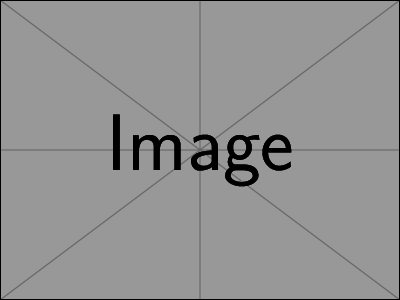
\includegraphics[width=100mm]{example-image}
	\caption{图片测试(最小宽度)\\Figure \ref{fig:1}\quad  Image test (Minimal width)\label{fig:1}}
\end{figure}

\begin{figure}[H]
	\centering
	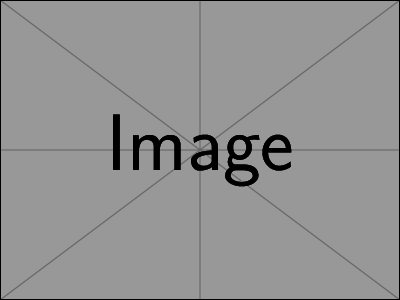
\includegraphics[width=130mm]{example-image}
	%\includegraphics[width=130mm]{./figures/你自己的图像文件}
	\caption{图片测试(最大宽度)\\Figure \ref{fig:2}\quad  Image test (Maximal width)\label{fig:2}}
\end{figure}

注意:这里为了减少图片上下的空白,使用了float宏包。


\newcommand{\bbb}{这是一个针对定理类环境进行的科技文稿排版测试}

\subsection{定理型环境示例}

\begin{definition} 
	这是一个针对定理类环境进行的科技文稿排版测试
\end{definition}

\begin{theorem}\label{th1}
	这是一个针对定理类环境进行的科技文稿排版测试
\end{theorem}

\begin{proof}
	这是一个针对定理类环境进行的科技文稿排版测试
\end{proof}

\begin{corollary}\label{cor1}
	这是一个针对定理类环境进行的科技文稿排版测试
\end{corollary}

\begin{lemma}\label{lem1}
	这是一个针对定理类环境进行的科技文稿排版测试
\end{lemma}

\begin{example}
	这是一个针对定理类环境进行的科技文稿排版测试
\end{example}

\subsection{脚注与引用}

\subsubsection{脚注}

这里是脚注测试\footnote{1111111111}这里是脚注测试这里是脚注测试这里是脚注测试\footnote{2222222222}这里是脚注测试这里是脚注测试这里是脚注测试这里是脚注测试这里是脚注测试这里是脚注测试这里是脚注测试这里是脚注测试这里是脚注测试这里是脚注测试这里是脚注测试这里是脚注测试这里是脚注测试这里是脚注测试这里是脚注测试\footnote{3333333333}这里是脚注测试这里是脚注测试这里是脚注测试这里是脚注测试这里是脚注测试这里是脚注测试这里是脚注测试这里是脚注测试这里是脚注测试这里是脚注测试这里是脚注测试这里是脚注测试

\subsubsection{定理类引用}

由定理\ref{th1}我们可以知道XXXXXXXX。

由引理\ref{lem1}我们可以知道XXXXXXXX。

由推论\ref{cor1}我们可以知道XXXXXXXX。

\subsubsection{文献引用的演示}

本模板使用biblatex进行文献管理,这是一套相对较新的系统。另外,使用了hushidong制作的符合gb7714-2015标准的biblatex样式。在此对他的工作表示感谢,要完成这样的样式非常不容易。本模板中gb7714-2015.bbx与gb7714-2015.cbx即为他的作品,在这里打包发布以便使用。详见\url{https://github.com/hushidong/biblatex-gb7714-2015}查找相关资料。

默认的bib文件位于\textasciitilde{}/reference/thesis-ref.bib,内容是由Wang
Tianshu制作,在此仅作演示之用。关于bib文件的编写与管理请自行查找相关教程。

默认的bib文件位于~/reference/thesis-ref.bib,内容是由Wang Tianshu制作,在此仅作演示之用。关于bib文件的编写与管理请自行查找相关教程。

下方的演示已经给出了正文中引用文献的基本方法,这与传统的cite命令是类似的。如有更多需求,请至\url{https://github.com/hushidong/biblatex-gb7714-2015}查找相关资料。

文献\parencite{Wuwei:2013}中提到xxxxxxx。

文献\parencite{zhouxu:2019}中提到yyyyyyy。

文献\parencite{tang:2008}中提到zzzzzzz。

\textcolor{blue}{\textbf{\uline{本模板使用parencite而不是cite命令,因为这样能与脚注所产生编号进行区分。当然,如果你没有脚注或尾注,那么cite命令也是推荐使用的。}}}


\nocite{*}

 %正文第三章

\chapter{总结与展望}\label{chap2}

概要回顾论文的主要结论,并提出一些展望。

本论文提供了一个完整的华东师范大学本科毕业论文模板. 这套模板符合
学校的有关要求, 方便易用. 这一工作对广大研究生更好地撰写学位论文无疑
带来很大的便利, 在其它场合同样会发挥重要的作用.  %正文第四章
\ClearPageStyle


%生成参考文献
\phantomsection
\setlength{\bibitemsep}{0pt}
\addcontentsline{toc}{chapter}{参考文献}
\printbibliography[title={\centerline{\bfseries\sffamily \zihao {-3}参考文献}}]
\ClearPageStyle


%生成附录
\phantomsection
\begin{appendix}
	\renewcommand{\chaptername}{附录 \Alph{chapter}}
	\renewcommand{\thesection}{\Alph{chapter}.\arabic{section}}
	\renewcommand{\thesubsection}{\Alph{chapter}.\arabic{section}.\arabic{subsection}}
	\renewcommand{\thesubsubsection}{\arabic{subsubsection}.}
	\renewcommand{\thetable}{\Alph{chapter}-\arabic{table}}
	\renewcommand{\theequation}{\Alph{chapter}-\arabic{equation}}
	\renewcommand{\thefigure}{\Alph{chapter}-\arabic{figure}}

\addtocontents{toc}{\setcounter{tocdepth}{2}}
\setcounter{subsection}{0}

%\ctexset { subsection = { name={,},number={\arabic{subsection}},format={\rmfamily \zihao {5}} } }
%\ctexset { subparagraph = { name={(,)},number={\arabic{subparagraph}},format={\rmfamily \zihao {5}},indent=2em } }


\chapter{附录标题}
\section{附录中的图形、表格、公式}

\subsection{公式}
附录中的公式(\ref{equ:Call})和(\ref{equ:Put})分别为:
\begin{equation}\label{equ:Call}
c=S_0N(d_1)-X e^{-r T}N(d_2)
\end{equation}
和
\begin{equation}\label{equ:Put}
p=X e^{-r T}N(-d_2)-S_0N(-d_1),
\end{equation}

\subsection{图形}
\begin{figure}[htbp!]
	\centering
	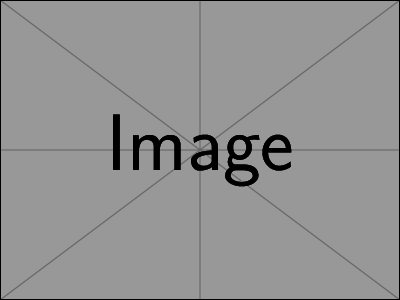
\includegraphics[width=100mm]{example-image}
	\caption{图片测试(最小宽度)\\Figure \ref{fig-a1}\quad  Image test (Minimal width)\label{fig-a1}}
\end{figure}

\subsection{表格}
\begin{table}[ht]
	\centering
	\caption{\label{tab-aa}Iris数据} 
	\begin{tabular}{rrrrrl}
		\toprule
		& Sepal.Length & Sepal.Width & Petal.Length & Petal.Width & Species \\ 
		\midrule
		1 & 5.10 & 3.50 & 1.40 & 0.20 & setosa \\ 
		2 & 4.90 & 3.00 & 1.40 & 0.20 & setosa \\ 
		3 & 4.70 & 3.20 & 1.30 & 0.20 & setosa \\ 
		4 & 4.60 & 3.10 & 1.50 & 0.20 & setosa \\ 
		5 & 5.00 & 3.60 & 1.40 & 0.20 & setosa \\ 
		6 & 5.40 & 3.90 & 1.70 & 0.40 & setosa \\ 
		\bottomrule
	\end{tabular}
\end{table}


\section{R代码}

\subsection{使用listings}
\begin{Rout}
	curve(dnorm(x), xlim=c(-4,4))
	curve(dnorm(x), xlim=c(-4,4))
	curve(dnorm(x), xlim=c(-4,4))
\end{Rout}

\section{Python代码}

% https://en.wikibooks.org/wiki/LaTeX/Source_Code_Listings

\subsection{使用listings}
\begin{pyout}[frame=single]
	import matplotlib.pyplot as plt
	import numpy as np
	x = np.arange(0.0, 6.0, 0.01)
	plt.plot(x, [x**2 for x in x])
	plt.show()
\end{pyout}



\subsection{使用pythonhighlight}
\begin{python}
	import matplotlib.pyplot as plt
	import numpy as np
	x = np.arange(0.0, 6.0, 0.01)
	plt.plot(x, [x**2 for x in x])
	plt.show()
\end{python}	

\end{appendix}

\ClearPageStyle


%生成感谢
\makeacknowledgement 

\end{document} 
